\documentclass[aspectratio=169]{beamer}
\usepackage[english,russian]{babel}
\usepackage[utf8]{inputenc}
\usepackage{verbatim}
\usepackage{graphicx}
\usepackage{pgfpages}
\usepackage{ulem}
\usepackage{float}
\usepackage{amsmath}

\setbeameroption{hide notes}

\setbeamercolor{title}{fg=white}
\setbeamercolor{author}{fg=white}
\setbeamercolor{normal text}{fg=black}
\setbeamercolor{frametitle}{fg=black}
\setbeamercolor{item}{fg=red}
\setbeamercolor{block title}{fg=red}
\setbeamercolor{section in toc}{fg=red}
\setbeamercolor{footline}{fg=white}
\setbeamercolor{title in head/foot}{fg=white,bg=black}

\setbeamertemplate{navigation symbols}{}
\setbeamertemplate{headline}{
    
\includegraphics[height=1mm, width=\paperwidth]{wg-headline.png}
}

\setbeamertemplate{footline}{
    \begin{beamercolorbox}[ht=1.2em]{title in head/foot}
        {\footnotesize \hspace{1em}\inserttitle, \insertshortauthor}
    \end{beamercolorbox}
}

\begin{document}

\title{IPv6 at home: NAT64, DNS64, OpenVPN}
\author{Maksim Melnikau}
\date{}

{
\title{
    \\
    {\Huge IPv6 at Home\\ \vspace{1em} NAT64, DNS64, OpenVPN}
    \\
}

\usebackgroundtemplate{
\includegraphics[width=\paperwidth]{wg-end.jpg}}
\begin{frame}[plain]{}
    \titlepage
\end{frame}
}

\begin{frame}[fragile]{IPv6}
\begin{block}{ifconfig eth0}
\begin{verbatim}Link encap:Ethernet HWaddr 52:54:00:03:c2:e6\end{verbatim} 
\begin{verbatim}inet addr:31.130.202.37 Bcast:31.130.202.63 Mask:255.255.255.192\end{verbatim}
\pause
\begin{verbatim}inet6 addr: fe80::5054:ff:fe03:c2e6/64 Scope:Link\end{verbatim}
\pause
\begin{verbatim}inet6 addr: 2001:67c:2268:1003:5054:ff:fe03:c2e6/64 Scope:Global\end{verbatim}
\end{block}
\end{frame}

\begin{frame}[fragile]{IPv6 in Belarus}
\begin{block}{Providers}
\begin{itemize}
\item MTS*
\item Velcom*
\item who else ?!
\end{itemize}
\end{block}

\begin{block}{host google.com}
\begin{verbatim}google.com has address 173.194.112.32
google.com has IPv6 address 2a00:1450:4001:801::1003\end{verbatim}
\end{block}
\end{frame}

\begin{frame}{VPS with IPv6 (1/2)}
    \begin{block}{Requirements}
        \begin{itemize}
        \item IPv6 andress
        \item subnet /64
        \item as closer as possible
        \end{itemize}
    \end{block}
    \pause
    \begin{block}{Advertisement}
        \begin{itemize}
        \item \url{http://www.datahata.by/} \par 
\includegraphics[width=0.3\textwidth]{datahata.png}
        \end{itemize}
    \end{block}
\end{frame}


\begin{frame}[fragile]{VPS with IPv6 (2/2)}
\begin{block}{ping6 -c 1 -n google.com}
\begin{verbatim}
PING google.com(2a00:1450:4001:c02::8a) 56 data bytes
64 bytes from 2a00:1450:4001:c02::8a: icmp_seq=1 ttl=55 time=46.5 ms

--- google.com ping statistics ---
1 packets transmitted, 1 received, 0% packet loss, time 0ms
rtt min/avg/max/mdev = 46.518/46.518/46.518/0.000 ms
\end{verbatim}
\end{block}

\end{frame}

\begin{frame}[fragile]{OpenVPN}
\begin{block}{/etc/openvpn/server.conf}
\begin{verbatim}
dev tun
tun-ipv6
push tun-ipv6
push "route-ipv6 2000::/3"
push "dhcp-option DNS 31.130.202.37"    # nat64/dns64
server-ipv6 2001:67c:2268:1007:1::/64
\end{verbatim}
\end{block}

\begin{block}{/etc/sysctl.conf}
\begin{verbatim}
net.ipv6.conf.all.forwarding=1
net.ipv6.conf.all.accept_ra=2
\end{verbatim}
\end{block}
\end{frame}

{
\usebackgroundtemplate{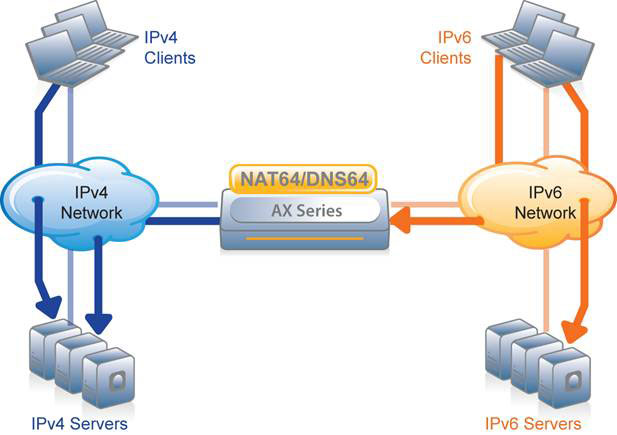
\includegraphics[height=\paperheight]{nat64.jpg}}
\begin{frame}[plain]{}
\end{frame}
}

\begin{frame}[fragile]{NAT64, DNS64 (2/3)}
\begin{block}{/etc/tayga.conf}
\begin{verbatim}
prefix 2001:67c:2268:1007:ffff::/96
\end{verbatim}
\end{block}

\begin{block}{/etc/bind/named.conf.options}
\end{block}
\begin{verbatim}
options {
        listen-on-v6 { any; };
        allow-query { any; };
        dns64 2001:67c:2268:1007:ffff::/96 {
                clients { any; };
        };
};
\end{verbatim}
\end{frame}

\begin{frame}[fragile]{NAT64, DNS64 (3/3)}
\begin{block}{host mlug.linux.by}
\begin{verbatim}
mlug.linux.by has address 216.59.3.46
mlug.linux.by has IPv6 address 2001:67c:2268:1007:ffff:0:d83b:32e
\end{verbatim}
\end{block}

\begin{block}{curl -6 -v 'http://mlug.linux.by'}
\begin{verbatim}
* Rebuilt URL to: http://mlug.linux.by/
* Hostname was NOT found in DNS cache
*   Trying 2001:67c:2268:1007:ffff:0:d83b:32e...
> GET / HTTP/1.1
... 
< HTTP/1.1 200 OK
...
\end{verbatim}
\end{block}
\end{frame}

\begin{frame}{Demo}
\end{frame}

\usebackgroundtemplate{
\includegraphics[width=\paperwidth]{wg-bg.jpg}}

{
\setbeamertemplate{footline}{}
\setbeamercolor{frametitle}{fg=white}
\setbeamercolor{normal text}{fg=white}
\setbeamercolor{block title}{fg=white}
\setbeamercolor{block body}{fg=red}

\usebackgroundtemplate{
\includegraphics[height=\paperheight]{wg-end.jpg}}
\begin{frame}{Thank You. Questions}
    \begin{block}{Maksim Melnikau}
    \par \url{mailto:maxposedon@gmail.com}
    \par \url{https://plus.google.com/+MaksimMelnikau}
    \par \url{http://en.wikipedia.org/wiki/IPv6}
    \par \url{https://community.openvpn.net/openvpn/wiki/IPv6}
    \par \url{https://ipvsix.me/?p=106}
    \par \url{http://www.datahata.by/}
    \end{block}
\end{frame}
}

\end{document}
